\documentclass[14pt,autoref,href,facsimile
%,fixint=false
%,times
]{disser}

\usepackage[a4paper,nohead,includefoot,mag=1000,
            margin=2cm,footskip=0.7cm]{geometry}
\usepackage{enumitem}
\usepackage[T2A]{fontenc}
\usepackage[utf8x]{inputenc}
\usepackage[english,russian]{babel}
\usepackage{tabularx}
\ifpdf\usepackage{epstopdf}\fi
% Поддержка нескольких списков литературы в одном документе
\usepackage{multibib}
% Создание команд для цитирования собственных работ диссертанта
% в отдельном разделе. В данном случае ссылка будет иметь вид \citemy{...}.
\newcites{my}{Список публикаций}

% Путь к файлам с иллюстрациями
\graphicspath{{figures/}}
\setlength{\parskip}{0ex}

\usepackage{amsmath}
\usepackage{amsmath,amssymb,amsthm}
\usepackage{multicol}
\usepackage{color}
%\usepackage{graphicx}
\usepackage{ucs}
\usepackage{pb-diagram}
\usepackage{enumerate}
\usepackage{appendix}
\usepackage{listings}
\usepackage{textcomp}


\definecolor{listinggray}{gray}{0.9}
\definecolor{lbcolor}{rgb}{0.9,0.9,0.9}
\lstset{
%	backgroundcolor=\color{lbcolor},
        language=Mathematica,
	tabsize=2,
	rulecolor=,
        basicstyle=\scriptsize,
        upquote=true,
%        aboveskip={1.5\baselineskip},
        columns=fixed,
        showstringspaces=false,
        extendedchars=true,
%        breaklines=true,
        prebreak = \raisebox{0ex}[0ex][0ex]{\ensuremath{\hookleftarrow}},
%        frame=single,
        showtabs=false,
        showspaces=false,
        showstringspaces=false,
        identifierstyle=\ttfamily,
        keywordstyle=\color[rgb]{0,0,1},
        commentstyle=\color[rgb]{0.133,0.545,0.133},
        stringstyle=\color[rgb]{0.627,0.126,0.941},
}

\newtheorem{statement}{Утверждение}
\newtheorem{theorem}{Теорема}
\newtheorem{axiom}{Аксиома}
\newtheorem{corollary}{Следствие}[chapter]
\newtheorem{lemma}{Лемма}
\newtheorem{mynote}{Замечание}[chapter]
%%\newtheorem{Def}{Definition}[section]
\newtheorem{Def}{Определение}[chapter]
\newtheorem{Cnj}[Def]{Гипотеза}
\newtheorem{Prop}{Свойство}
%%\newtheorem{example}{Example}[section]

\theoremstyle{definition}
\newtheorem{definition}{Определение}
\newtheorem{remark}{Замечание}[chapter]
\newtheorem{example}{Пример}[chapter]
\newtheorem{exercise}{Упражнение}
\newtheorem{conjecture}{Гипотеза}[chapter]

\newcommand{\go}{\stackrel{\circ }{\mathfrak{g}}}
\newcommand{\ao}{\stackrel{\circ }{\mathfrak{a}}}
\newcommand{\co}[1]{\stackrel{\circ }{#1}}
\newcommand{\pia}{\pi_{\mathfrak{a}}}
\newcommand{\piab}{\pi_{\mathfrak{a}_{\perp}}}
\newcommand{\gf}{\mathfrak{g}}
\newcommand{\af}{\mathfrak{a}}
\newcommand{\uf}{\mathfrak{u}}
\newcommand{\sfr}{\mathfrak{s}}
\newcommand{\aft}{\widetilde{\mathfrak{a}}}
\newcommand{\afb}{\mathfrak{a}_{\perp}}
\newcommand{\hf}{\mathfrak{h}}
\newcommand{\hfb}{\mathfrak{h}_{\perp}}
\newcommand{\pf}{\mathfrak{p}}

\newcommand{\gfh}{\hat{\mathfrak{g}}}
\newcommand{\afh}{\hat{\mathfrak{a}}}
\newcommand{\bff}{\mathfrak{b}}
\newcommand{\hfg}{\hf_{\gf}}

%\renewcommand{\thestatement}{}

\begin{document}
% Включение файла с общим текстом диссертации и автореферата
% (текст титульного листа и характеристика работы).


% Общие поля титульного листа диссертации и автореферата
\institution{Санкт-Петербургский Государственный Университет}

\topic{Правила ветвления аффинных алгебр Ли\\ и приложения в моделях конформной теории поля}

\author{Назаров Антон Андреевич}

\specnum{01.04.02}
\spec{Теоретическая физика}

\sa{Ляховский Владимир Дмитриевич}
\sastatus{д.~ф.-м.~н., проф.}

\city{Санкт-Петербург}
\date{\number\year}

% Общие разделы автореферата и диссертации

\mkcommonsect{actuality}{Актуальность работы}{%

  Последние тридцать лет конформная теория поля в двух измерениях привлекает большое внимание исследователей. Эта теория используется для описания критического поведения в двумерных статистических системах. Благодаря наличию бесконечномерной алгебры симметрии двумерная конформная теория поля может быть сформулирована аксиоматически. Помимо математической красоты теория обладает огромной практической ценностью -- с ее использованием было получено большое количество результатов и численных предсказаний в изучении критического поведения в двумерных системах \cite{difrancesco1997cft,henkel1999conformal}. Методы двумерной конформной теории поля с успехом применяются также при изучении эффекта Кондо \cite{cox1998exotic,affleck1993exact} и дробного квантового эффекта Холла \cite{moore1991nonabelions}. 

Поиски строгого математического доказательства для предсказаний двумерной конформной теории поля \cite{cardy1992critical} в последние годы привели к большому количеству новых идей и результатов в дискретном комплексном анализе \cite{smirnov2001critical,duminil2011conformal,smirnov2010discrete}.

Теория представлений бесконечномерных алгебр Ли является важным инструментом изучения моделей конформной теории поля. Помимо алгебры Вирасоро, наличие которой обязательно в двумерной конформной теории поля, большую роль играют аффинные алгебры Ли. Изучение аффинных алгебр Ли было начато Виктором Кацем и Робертом Муди в 1960-х годах с попытки обобщения классификации простых конечномерных алгебр Ли на бесконечномерный случай \cite{kac1968simple,moody1968new}. Первоначально интерес к этим алгебрам был связан с модулярными свойствами характеров их модулей \cite{kac1984infinite,macdonald1971affine}. После возникновения двумерной конформной теории поля были предложены модели Весса-Зумино-Новикова-Виттена \cite{witten1984nab}, а затем и coset-модели \cite{Goddard198588}, в которых теория представлений аффинных алгебр Ли играет определяющую роль. 

Моделям Весса-Зумино-Новикова-Виттена, coset-моделям и теории представлений аффинных алгебр Ли  посвящены тысячи работ. Однако многие проблемы по-прежнему не имеют простых решений. Например, задача вычисления коэффициентов ветвления для представлений алгебр Ли стоит уже многие десятилетия. Она актуальна для различных физических приложений в coset-моделях конформной теории поля. При этом, в отличие от проблемы вычисления кратностей весов, для вычисления коэффициентов ветвления не существовало особенно эффективных алгоритмов. 
}

  
\mkcommonsect{objective}{Цели и задачи работы}{%
 Разработка рекуррентного подхода к функциям ветвления аффинных алгебр Ли, его связь с проблемами теории представлений и его приложения в моделях конформной теории поля.
}
 
\mkcommonsect{novelty}{Научная новизна и практическая значимость.}{%
  В диссертации впервые решены следующие задачи:
  \begin{itemize}%%[topsep=0pt, itemsep=-1ex]
  \item Получено эффективное рекуррентное соотношение для коэффициентов ветвления модулей аффинных и конечномерных алгебр Ли на модули не максимальных подалгебр.   Алгоритм вычисления коэффициентов ветвления реализован в пакете  {\bf Affine.m} для популярной системы компьютерной алгебры {\it Mathematica}.
  \item Установлена прямая связь инъективного сплинта и ветвлений. Доказано, что при определенных условиях  кратности весов вспомогательного модуля иньективного сплинта совпадают с коэффициентами ветвления в редукции на вложенную подалгебру. Наличие расщепления приводит к существенному упрощению при вычислении коэффициентов ветвления. 
%  \item Показано, что наличие расщепления приводит к существенному упрощению при вычислении коэффициентов ветвления.
  \item Исследована связь процедуры редукции с обобщенной резольвентой Бернштейна-Гельфанда-Гельфанда (БГГ).  Показано, что разложение сингулярного элемента определяет как коэффициенты ветвления, так и обобщенную БГГ-резольвенту, так как действие веера вложения на компоненты разложения порождает обобщенные модули Верма, которые образуют точную последовательность.
  \item Построена модель обобщенного стохастического процесса Шрамма-Лёвнера для систем с калибровочной инвариантностью, соответствующих coset-моделям конформной теории поля.
  \end{itemize}
Отметим, что  пакет {\bf Affine.m} может быть использован для решения задач теории представлений конечномерных и аффинных алгебр Ли, возникающих в различных областях физики, начиная от изучения атомных и молекулярных спектров и заканчивая конформной теорией поля и интегрируемыми системами.
}
 
%\mkcommonsect{value}{Практическая значимость}

\mkcommonsect{results}{На защиту выносятся следующие результаты и положения:}{%
\begin{itemize}%%[topsep=0pt, itemsep=-1ex]
\item Получены новые рекуррентные соотношения на коэффициенты ветвления представлений аффинных алгебр Ли на представления произвольных редуктивных подалгебр, с использованием разложения сингулярных элементов
\item Установлено, что разложение сингулярного элемента определяет как коэффициенты ветвления, так и обобщенную БГГ-резольвенту, так как действие веера вложения на компоненты разложения порождает обобщенные модули Верма, которые образуют точную последовательность
\item  Доказано, что при определенных условиях  кратности весов вспомогательного модуля иньективного сплинта совпадают с коэффициентами ветвления в редукции на вложенную подалгебру. Наличие расщепления приводит к существенному упрощению при вычислении коэффициентов ветвления.
\item Показано, что условие для мартингала, определяющее классификацию операторов изменения граничных условий в наблюдаемых стохастического процесса Шрамма-Лёвнера, задает ограничения на структуру сингулярных элементов представлений аффинной алгебры Ли, порожденных граничными состояниями. Изучение структуры сингулярных элементов существенно упрощает поиск операторов смены граничных условий. Построена модель обобщенного стохастического процесса Шрамма-Лёвнера для систем с калибровочной инвариантностью, соответствующих coset-моделям конформной теории поля и показано, что такое обобщение совместно с coset-реализацией минимальных моделей.
%\item Продемонстрирована роль сингулярных элементов в построении мартингалов стохастического процесса Шрамма-Лёвнера, то есть проиллюстрировано применение алгебраических методов теории представлений аффинных алгебр Ли в изучении критического поведения в двумерных решеточных моделях
\item Разработан пакет программ {\bf Affine.m}, реализующий различные алгоритмы для вычислений в теории представлений конечномерных и аффинных алгебр Ли
\end{itemize}

}

\mkcommonsect{approbation}{Апробация работы}{%
  Материалы диссертации докладывались на трех международных конференциях, а также на семинарах кафедры физики высоких энергий и элементарных частиц СПбГУ, на семинарах в лаборатории имени П.Л. Чебышева математико-механического факультета СПбГУ, на семинаре лаборатории теоретической физики ОИЯИ (Дубна).

%  международном семинаре молодых ученых ``Workshop on Advanced Computer Simulation Methods''  27 - 29 апреля 2009 
%(Санкт-Петербург),  на международных конференциях:  ``Модели квантовой теории поля (MQFT-2010)'' 18-22 октября 2010 
%(Санкт-Петербург), ``Supersymmetries and Quantum Symmetries - 2011'', 18-23 июля 2011 (Дубна), ``Quantum Theory and 
%Symmetries (QTS-7)'', 7-13 августа 2011 (Прага). 
}

\mkcommonsect{pub}{Публикации.}{%
Материалы диссертации опубликованы в $10$ печатных работах, из них $5$ статей в
рецензируемых журналах~\citemy{2010arXiv1007.0318L,2011arXiv1102.1702L,2011arXiv1111.6787L,NazarovJETPletters,2011arXiv1107.4681N}, $5$ статей в
сборниках тезисов и трудов конференций \citemy{2011arXiv1112.4354N,2010LyakhovskyNazarovMQFT,Nazarov2008,NazarovACSM2009,2012arXiv1204.1855L}.
}

\mkcommonsect{contrib}{Личный вклад автора.}{%
  Все основные результаты и выносимые на защиту положения получены автором самостоятельно. Личный вклад автора в работы с соавтором составляет $50$ процетнов, в работы без соавторов -- $100$ процентов. 
}

\mkcommonsect{struct}{Структура и объем диссертации}{%
Диссертация состоит из введения и пяти глав, содержит 160 страниц и 30 рисунков. Список литературы включает 151 наименование. 

}

%%  \mkcommonsect{content}{Содержание работы}{%
%%  
%%  }

%%
%% End of file
%%% Local Variables: 
%%% mode: latex
%%% TeX-master: "thesis"
%%% End: 


\title{АВТОРЕФЕРАТ\\
диссертации на соискание ученой степени\\
кандидата физико-математических наук}

\maketitle

% Внутренняя сторона обложки
\noindent
\begin{center}
Работа выполнена в Санкт-Петербургском государственном университете.
% \emph{название организации}.
\end{center}
\vskip1ex
\begin{tabularx}{\linewidth}{lp{1cm}X}
Научный руководитель:  & & \emph{доктор физико-математических наук}, \\
                       & & \emph{профессор}, \\
                       & & \emph{Ляховский Владимир Дмитриевич} \\
Официальные оппоненты: & & \emph{Кулиш Петр Петрович}\\
                       & & \emph{доктор физико-математических наук}, \\
                       & & \emph{профессор},\\
                       & & \emph{Санкт-Петербургское   отделение
Математического   института   им.  В.А. Стеклова   РАН, главный научный сотрудник, заведующий 
лаборатории математических проблем физики}; \\
                       & & \emph{Мудров Андрей Игоревич} \\
                       & & \emph{кандидат физико-математических наук, Университет Лестера (Великобритания), преподаватель} 
\\
Ведущая организация:   & & \emph{Объединенный институт ядерных исследований}\\
\end{tabularx}

\vskip2ex\noindent
Защита состоится \datefield{} в \rule[0pt]{1cm}{0.5pt}\, часов
на заседании диссертационного совета \emph{Д 212.232.24}  при \emph{Санкт-Петербургском государственном университете} по адресу:
\emph{199004, Санкт-Петербург, Средний пр. В.О., д. 41/43, ауд. 304}

\vskip1ex\noindent
С диссертацией можно ознакомиться в библиотеке
\emph{Санкт-Петербургского государственного университета}.

%\vskip1ex
\noindent
Автореферат разослан \datefield{}

%\vskip2ex\noindent
%Отзывы и замечания по автореферату в двух экземплярах, заверенные
%печатью, просьба высылать по вышеуказанному адресу на имя ученого секретаря
%диссертационного совета.

\vfill
\noindent
Ученый секретарь\\
диссертационного совета,%\\
%\emph{д.ф.-м.н.}%, \emph{ученое звание}%
\hfill
\makeatletter
% вставка файла, содержащего факсимиле ученого секретаря
\ifDis@facsimile
  \raisebox{-4pt}{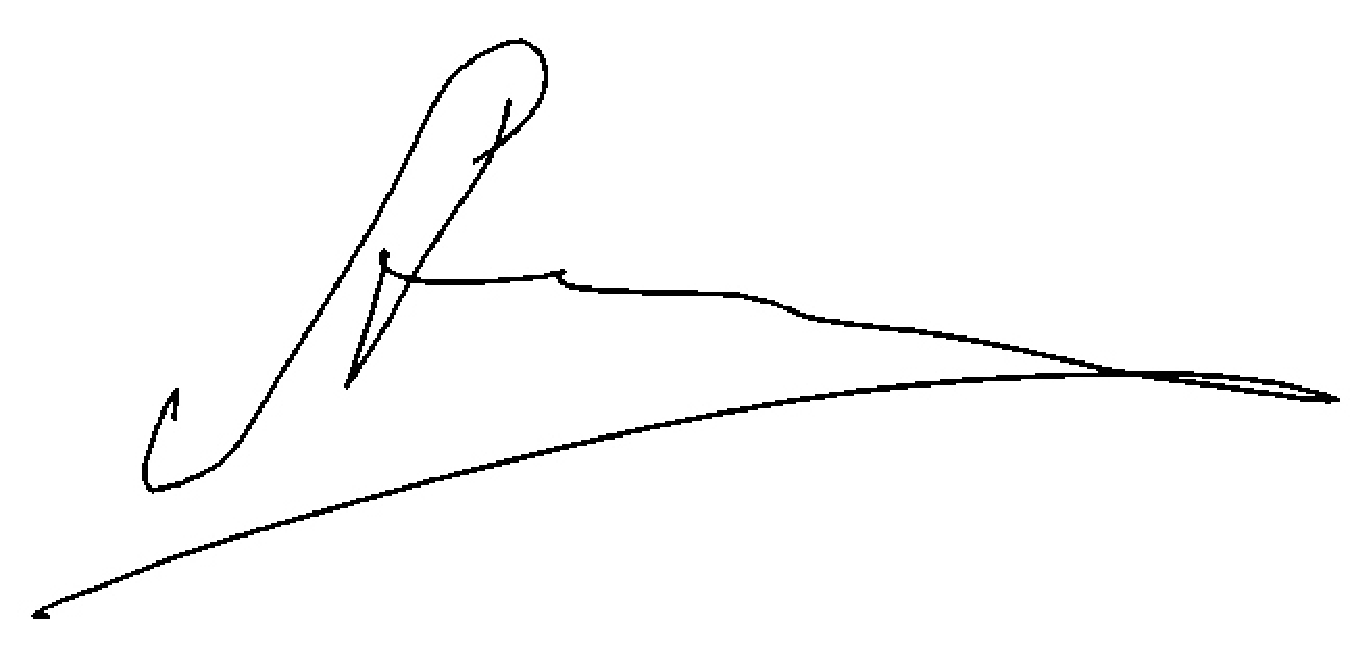
\includegraphics[width=3cm,height=1cm]{aksenova}}\hfill
\fi%
\makeatother%
\emph{Аксенова Е.В.}

\clearpage

\nsection{Общая характеристика работы}

% Актуальность работы
%\actualitysection
%\actualitytext

\textbf{Актуальность работы.}
Последние тридцать лет конформная теория поля в двух измерениях привлекает большое внимание исследователей. Конформная теория поля используется для описания критического поведения в двумерных статистических системах и  обладает большой практической ценностью -- с ее использованием было получено значительное количество результатов и численных предсказаний. Методы двумерной конформной теории поля с успехом применяются также при изучении эффекта Кондо и дробного квантового эффекта Холла. Благодаря наличию бесконечномерной алгебры симметрии двумерная конформная теория поля может быть сформулирована аксиоматически. 

Поиски строгого математического доказательства для предсказаний двумерной конформной теории поля в последние годы привели к большому количеству новых идей и результатов в дискретном комплексном анализе \cite{smirnov2001critical}.

Теория представлений бесконечномерных алгебр Ли является важным инструментом изучения моделей конформной теории поля. Помимо алгебры Вирасоро, наличие которой обязательно в двумерной конформной теории поля, большую роль играют аффинные алгебры Ли. Изучение аффинных алгебр Ли было начато Виктором Кацем и Робертом Муди в 1960-х годах с попытки обобщения классификации простых конечномерных алгебр Ли на бесконечномерный случай \cite{kac1968simple,moody1968new}. Интерес к этим алгебрам был связан с модулярными свойствами характеров их модулей. После возникновения двумерной конформной теории поля были предложены модели Весса-Зумино-Новикова-Виттена (ВЗНВ), а затем и coset-модели, в которых теория представлений аффинных алгебр Ли играет определяющую роль. 

ВЗНВ-моделям, coset-моделям и теории представлений аффинных алгебр Ли  посвящены тысячи работ. Однако многие проблемы по-прежнему не имеют простых решений. Так, задача вычисления коэффициентов ветвления для представлений алгебр Ли стоит уже многие десятилетия. Она актуальна для физических приложений в coset-моделях конформной теории поля. Для вычисления коэффициентов ветвления, в отличие от проблемы нахождения кратностей весов, не существовало особенно эффективных алгоритмов. 



% Цель диссертационной работы
%\objectivesection
%\objectivetext

% Научная новизна
\noveltysection
\noveltytext

% Практическая значимость
%\valuesection
%\valuetext

% Результаты и положения, выносимые на защиту

\resultssection
\resultstext

% Апробация работы
\approbationsection
\approbationtext

% Публикации
\pubsection
\pubtext

% Личный вклад автора
\contribsection
\contribtext

% Структура и объем диссертации
\structsection
\structtext

% \contentsection
% \contenttext


\vspace{-0.5cm}
\nsection{Содержание работы}
\vspace{-0.3cm}
\textbf{Во Введении} обоснована актуальность диссертационной работы,
сформулирована цель и аргументирована научная новизна исследований, показана
практическая значимость полученных результатов, представлены выносимые на
защиту научные положения.

\textbf{Глава 1} носит обзорный характер. В ней приводится аксиоматическая формулировка конформной теории поля, описываются ВЗНВ-модели и coset-модели. Затем демонстрируется роль аффинных алгебр в описании этих моделей и вводятся основные понятия теории представлений, использующиеся в диссертации. Мы указываем на то, что основные свойства интегрируемых модулей старшего веса определяются структурой сингулярного элемента, что выражается в формуле Вейля-Каца для формальных характеров. Мы обсуждаем конформную теорию поля на области с границей, так как она оказывается связана со стохастическим описанием решеточных моделей. 

\textbf{В главе 2} выводится основное рекуррентное соотношение на коэффициенты ветвления. Сначала доказывается лемма о разложении сингулярного элемента. Структура сингулярного элемента определяет свойства модуля алгебры Ли, поэтому разложение определяет правила ветвления и позволяет сформулировать рекуррентную процедуру редукции. Основные результаты данной главы опубликованы в работе \citemy{2010arXiv1007.0318L}. 

Формула Вейля-Каца для формальных характеров интегрируемых модулей старшего веса конечномерных и аффинных алгебр Ли имеет вид $\mathrm{ch} V^{(\mu)} = \frac{\Psi^{(\mu)}}{R}$,
где $\Psi^{(\mu)}$ -- сингулярный элемент модуля, а $R=\prod_{\alpha\in \Delta^+}(1-e^{-\alpha})^{\mathrm{mult}(\alpha)}$ -- знаменатель Вейля. Здесь $\Delta^+$ -- множество положительных корней алгебры, а $\rho$ -- вектор Вейля. Сингулярный элемент определяется набором сингулярных весов модуля и имеет разный вид для разных типов модулей старшего веса. Например, $\Psi^{(\mu)}=\sum_{w\in W} \epsilon(w) e^{w(\mu+\rho)-\rho}$ для неприводимых модулей ($W$ -- группа Вейля). Знаменатель  Вейля $R$ является универсальным объектом, характеризующим корневую систему алгебры Ли, а свойства модуля определяются сингулярным элементом.

Процедура редукции состоит в разложении модуля алгебры Ли $\gf$ в сумму модулей некоторой подалгебры $\af$:
$ L_{\gf\downarrow \af}^{\mu }=\bigoplus
\limits_{\nu \in P_{\af}^{+}}b_{\nu }^{\left( \mu \right) }L_{\af}^{\nu }.$

Используя оператор проекции  $\pi_{\af}$ (на весовое пространство $\hf_{\af}^*$), перепишем это разложение для формальных характеров: 
\begin{equation}
\label{branching1}
 \pi _{\af}\circ ch\left( L^{\mu }\right)
 =\sum_{\nu \in P_{\af}^{+}}b_{\nu }^{(\mu)}ch\left( L_{\af}^{\nu }\right) .
\end{equation}
Нас интересуют коэффициенты ветвления $b^{(\mu)}_{\nu}$.

Для любой алгебры $\gf$ и подалгебры $\af\subset \gf$ можно построить  подалгебру $\afb$ такую, что $\Delta _{\af_{\perp }} =\left\{ \beta \in \Delta _{\gf}| \forall h \in \hf_{\af};  \beta\left(h \right)=0  \right\}$.

Обозначим через $W_{\afb}$ подгруппу группы Вейля $W$, порожденную отражениями $w _{\beta }$, соответствующими корням $\beta \in \Delta _{\afb}^{+}$ . Подсистема  $\Delta _{\af_{\perp }}$ определяет подалгебру $\af_{\perp }$ с подалгеброй Картана $\hf_{\afb}$.  

Пусть
$\hf_{\perp }^{\ast }:=\left\{ \eta \in \hf_{\perp \af}^{\ast
}|\forall h \in \hf_{\af\oplus \af_{\perp}}; \eta \left( h \right)=0 \right\}$, тогда имеет место разложение подалгебры Картана $\hf=\frak{\hf_{\af}}\oplus \hf_{\afb}\oplus\hf_{\perp }$.
Для подалгебр из ортогональной пары  $\left( \af,\afb\right) $ рассмотрим соответствующие векторы Вейля $\rho _{\af}$ и $\rho _{\af_{\perp }}$, и образуем так называемые  ``дефекты'' вложения $\mathcal{D}_{\af}:=\rho _{\af}-\pi _{\af}\rho$, $\mathcal{D}_{\af_{\perp }}:=\rho _{\af_{\perp }}-\pi_{\afb}\rho$.

Рассмотрим сингулярные веса  $\left\{\left( w(\mu +\rho )-\rho \right)|w  \in W \right\}$  модуля старшего веса  $L_{\gf}^{\mu }$ и их проекции на $h_{\widetilde{\af_{\perp }}}^{\ast }$ (дополнительно сдвинутые на дефект $-\mathcal{D}_{\af_{\perp }}$):
\begin{equation*}
\mu _{\widetilde{\af_{\perp }}}\left( w\right) :=\pi _{\widetilde{\frak{%
a}_{\perp }}}\circ\left[ w(\mu +\rho )-\rho \right] -\mathcal{D}_{\af_{\perp
}},\quad w\in W.
\end{equation*}
Среди весов  $\left\{\mu _{\widetilde{\af_{\perp }}}\left( w\right)|w\in W\right\}$ выберем находящиеся в главной камере Вейля $\overline{C_{\widetilde{\afb}}}$. Множество $U:=\left\{ u\in W|\quad \mu _{\widetilde{\af_{\perp }}}\left( u\right)
\in \overline{C_{\widetilde{\af_{\perp }}}}\right\}$ состоит из элементов группы Вейля, переводящих старший вес в главную камеру Вейля подалгебры $\tilde\afb$ (с учетом сдвига на $\rho$ и на дефект). Элементы $U$ являются представителями классов смежности $W/W_{\af_{\perp }}$. 
Каждому элементу  $U$ поставим в соответствие вес $\mu _{\af}\left( u\right) :=\pi _{\af}\circ\left[ u(\mu +\rho )-\rho \right] +\mathcal{D}_{\afb}$. Аналогичным образом определим $\mu _{\tilde \af}\left( u\right) :=\pi _{\tilde \af}\left[ u(\mu +\rho )-\rho \right] +\mathcal{D}_{\afb}$ и $\mu _{\afb}\left( u\right) :=\pi _{\afb}\left[ u(\mu +\rho )-\rho \right] +\mathcal{D}_{\afb}$. Мы доказываем следующую лемму о разложении сингулярного элемента:
\vspace{-0.3cm}
\begin{lemma}
\label{lemma}
Пусть $\left( \af,\afb \right)$ -- ортогональная пара редуктивных подалгебр $\gf$ и  $\widetilde{\afb}=\afb\oplus \hf_{\perp }$, $\widetilde{\af}=\af\oplus\hf_{\perp }$ ,
$L^{\mu }$ -- модуль старшего веса с сингулярным элементом $\Psi ^{\left(\mu \right)}$ ,
$R_{\af_{\perp }}$ -- знаменатель Вейля для подалгебры $\af_{\perp }$.
Тогда элемент  $\Psi ^{\left( \mu \right) }_{\left(  \af, \afb \right)}=\pi _{\af}\left( \frac{\Psi _{\gf}^{\mu }}{R_{\af_{\perp }}}\right) $ можно разложить в сумму по  $u\in U$ сингулярных весов $e^{\mu _{\af}\left( u\right) }$ с коэффициентами $\epsilon (u)\mathrm{\dim}\left( L_{\widetilde{\afb}}^{\mu _{\widetilde{\afb}}\left( u\right) }\right) $:
\begin{equation}
\Psi ^{\left( \mu \right) }_{\left(  \af, \afb \right)}=\quad \pi _{\af}\left( \frac{\Psi^{\mu }}{R_{\af%
_{\perp }}}\right) =\sum_{u\in U}\;\epsilon (u)\mathrm{\dim }
\left( L_{\widetilde{\af_{\perp }}}^{\mu _{%
\widetilde{\af_{\perp }}}\left( u\right) }\right) e^{\mu _{\af}\left( u \right) }.
\end{equation}
\end{lemma}
Введем ``веер вложения'', который необходим для формулировки рекуррентных соотношений:
\vspace{-0.5cm}
\begin{definition}
\label{fan-definition} Рассмотрим произведение
\begin{equation}
\prod_{\alpha \in \Delta ^{+}\setminus \Delta _{\afb }^{+}}\left( 1-e^{-\pi
_{\af}\alpha }\right) ^{\mathrm{mult}(\alpha )-\mathrm{mult}_{\af%
}(\pi _{\af}\alpha )}=-\sum_{\gamma \in P_{\af}}s(\gamma
)e^{-\gamma }  \label{eq:142}
\end{equation}
и носитель $\Phi _{\af\subset \gf}\subset P_{\af}$ функции $s(\gamma )=\det \left( \gamma \right) $ : \quad
$
\Phi _{\af\subset \gf}=\left\{ \gamma \in P_{\af}|s(\gamma
)\neq 0\right\}   \label{eq:37}
$
Упорядочение корней в  $\Delta _{\af}$ индуцирует естественное упорядочение весов в $P_{\af}$. Обозначим через $\gamma_{0}$ наименьший вектор $\Phi _{\af\subset \gf}$. 

Множество
$\Gamma _{\af\rightarrow \gf}=\left\{ \xi -\gamma _{0}|\xi \in \Phi _{%
\af\subset \gf}\right\} \setminus \left\{ 0\right\}$
называется  \textit{веером вложения}.
\end{definition}\vspace{-0.3cm}
Веер вложения универсален и зависит только от вложения $\af\to\gf$ и не зависит от модуля $L^{(\mu)}$.

Введем сингулярные коэффициенты ветвления следующим образом:
\begin{equation*}
  \label{eq:3}
  \begin{array}{l}
  k^{(\mu)}_{\xi}=b^{(\mu)}_{\xi} \quad\text{если}\quad \xi\in \bar C_{\af}\\
  k^{(\mu)}_{\xi}=\epsilon(w) b^{(\mu)}_{w(\xi+\rho_{af})-\rho_{\af}} \quad\text{где}\; w\in W_{\af}:w(\xi+\rho_{\af})-\rho_{\af}\in \bar C_{\af}.
  \end{array}
\end{equation*}

Теперь можно сформулировать основную теорему, которая позволяет рекуррентно вычислять коэффициенты ветвления.
\vspace{-0.5cm}
\begin{theorem}
  Для сингулярных коэффициентов ветвления $k^{(\mu)}_{\nu}$ выполняется соотношение
  \begin{equation}
    \label{recurrent-relation}
    \begin{array}{c}
      k_{\xi }^{\left( \mu \right) }=-\frac{1}{s\left( \gamma _{0}\right) }\left(
        \sum_{u\in U} \epsilon(u)\;
        \dim \left( L_{\widetilde{\af_{\perp }}}^{\mu
        _{\widetilde{\af_{\perp }}}\left( u\right) }\right)
        \delta_{\xi-\gamma_0,\pi_{\af}(u(\mu+\rho)-\rho)}+ \right.\\
      \left.
        +\sum_{\gamma \in
          \Gamma _{\af \rightarrow \gf}}s\left( \gamma +\gamma _{0}\right) k_{\xi
          +\gamma }^{\left( \mu \right) }\right).
    \end{array}
  \end{equation}
\end{theorem}
Далее мы анализируем пары $(\af,\afb)$ для простых алгебр Ли. Оказывается, что для ``ортогональной пары'' $(\af,\afb)$, вообще говоря, $\af\oplus\afb\not\subset\gf $. В частности, для серии простых конечномерных алгебр $B_n$ существуют ``ортогональные пары'' подалгебр $(B_k,B_{n-k})$.

На основании рекуррентного соотношения (\ref{recurrent-relation}) сформулирован алгоритм вычисления коэффициентов ветвления. Остальные разделы главы 2 содержат примеры вычислений с использованием предложенного алгоритма, а также описание роли функций ветвления в формулировке конформной теории поля на торе и в coset-моделях конформной теории поля. 

\textbf{В главе 3} мы используем  разложение сингулярного элемента, чтобы показать связь ветвления с (обобщенной) БГГ-резольвентой.  Данные результаты опубликованы в работах \citemy{2011arXiv1102.1702L,2010LyakhovskyNazarovMQFT}.

Для полупростой конечномерной алгебры $\gf$  и полупростой конечномерной подалгебры $\af$ алгебра $\afb$ является регулярной. Отношение знаменателей Вейля порождает параболические модули Верма. Сингулярный элемент  $\Psi ^{\left( \mu \right) }$ может быть разложен в сумму по  $u\in U$  сингулярных элементов $\Psi _{\afb}^{\mu _{\afb}\left( u\right) }$ с коэффициентами
$\epsilon (u)e^{\mu _{\widetilde{\af}}\left( u\right) }$:
\begin{equation}
\Psi ^{\left( \mu \right) }=\sum_{u\in U}\;\epsilon (u)e^{\mu _{\widetilde{%
\mathfrak{a}}}\left( u\right) }\Psi _{\frak{a}_{\perp }}^{\mu _{\frak{a}%
_{\perp }}\left( u\right) }.  \label{sing decomp main}
\end{equation}
Мы доказываем следующее утверждение, демонстрирующее, что разложение сингулярного элемента связано с разложением характера неприводимого модуля в комбинацию характеров обобщенных модулей Верма
\vspace{-0.3cm}
\begin{statement}
%\bigskip
Для ортогональной подалгебры  $\frak{a}_{\perp }$ в $\frak{g}$ (являющейся ортогональным партнером редуктивной подалгебры $\frak{a}\hookrightarrow \frak{g}$) характер интегрируемого модуля старшего веса  $L^{\mu }$ может быть представлен в виде комбинации (с целочисленными коэффициентами) характеров параболических модулей Верма, распределенных по множеству весов $\mu _{\widetilde{\mathfrak{a}}}\left(
u\right)$:
\begin{equation}
\mathrm{ch}\left( L^{\mu }\right) =\sum_{u\in U}\;\epsilon (u)e^{\mu _{%
\widetilde{\frak{a}}}\left( u\right) }\mathrm{ch}M_{I}^{\mu _{\frak{a}%
_{\perp }}\left( u\right) },  \label{gen Weyl-Verma}
\end{equation}
где  $U:=\left\{ u\in W|\quad \mu _{\frak{a}_{\perp }}\left( u\right) \in
\overline{C_{\frak{a}_{\perp }}}\right\} $ и $I$ -- такое подмножество в  $S$, что $\Delta _{I}^{+}$ эквивалентно $\Delta _{\frak{a}_{\perp }}^{+}$.
\end{statement}
\vspace{-0.3cm}
Связь редукции и (обобщенной) резольвенты БГГ дается следующим утверждением:
\vspace{-0.3cm}
\begin{statement}
Пусть $L^{\mu }$ --  $\frak{g}$-модуль со старшим весом $\mu \in P^{+}$, и пусть регулярная подалгебра  $\afb\hookrightarrow \frak{g}$ является ортогональным партнером редуктивной подалгебры $\frak{a}\hookrightarrow \frak{g}$. Тогда разложение (\ref{sing decomp main}) определяет как обобщенную резольвенту $L^{\mu }$ по отношению к $\afb$, так и правила ветвления $L^{\mu }$ по отношению к $\afb$, так и правила ветвления $L^{\mu }$ по отношению к $\af$ .
\end{statement}
\vspace{-0.3cm}
\textbf{Глава 4} посвящена сплинтам -- расщеплением корневой системы алгебры Ли в объединение образов корневых систем двух алгебр, не обязательно являющихся подалгебрами данной алгебры. Если одна из алгебр является подалгеброй, то сплинт приводит к резкому упрощению в вычислении коэффициентов ветвления -- они совпадают с кратностями весов в модуле другой алгебры. Основная часть главы посвящена доказательству этого факта. Кроме того, сплинт корневой системы простой конечномерной алгебры Ли приводит к возникновению новых соотношений на струнные функции и функции ветвления соответствующего аффинного расширения. Эти соотношения обсуждаются в разделе 4.4.
Данные результаты опубликованы в статьях \citemy{2011arXiv1111.6787L,2012arXiv1204.1855L}.

\vspace{-0.3cm}
\begin{definition}
Пусть $\Delta _{0}$ и $\Delta$ -- корневые системы с соответствующими весовыми решетками $P_{0}$ и $P$. Отображение $\phi :\left\{
\Delta _{0}\hookrightarrow \Delta , 
P_{0}\hookrightarrow P
\right\}
$ называется ``вложением'', если  $\phi$ вкладывает $\Delta _{0}$ в $\Delta $ и действует гомоморфно по отношению к группам сложения векторов в $P_{0}$ и $P$:
$
\phi (\gamma )=\phi (\alpha )+\phi (\beta )
$
для любой тройки $\alpha ,\beta ,\gamma \in P_{0}$, такой, что $\gamma =\alpha+\beta $.
\end{definition}
\vspace{-0.5cm}
Вложение $\phi$ индуцирует вложение формальных алгебр: ${\mathcal{E}}_0\hookrightarrow \mathcal{E}$ и для образа ${\mathcal{E}}_i=\mathrm{Im}_{\phi}\left( {\mathcal{E}}_0\right)$ можно рассмотреть обратное отображение $\phi^{-1}:{\mathcal{E}}_i \longrightarrow {\mathcal{E}}_0$. Нужно различать два класса вложений: ``метрические'', если скалярное произведение (заданное формой Киллинга) в корневом пространстве $P_0$ инвариантно по отношению к  $\phi$ и ``неметрические'', если оно не  $\phi$-инвариантно. 

Будем говорить, что корневая система $\Delta$ ``расщепляется'' на  $(\Delta _{1},\Delta _{2})$, если существует два вложения  $\phi _{1}:\Delta _{1}\hookrightarrow \Delta $ и $\phi _{2}:\Delta _{2}\hookrightarrow \Delta $, где (a) $\Delta $ -- несвязное объединение образов $\phi _{1}$ и $\phi _{2}$, и (b) ни ранг  $\Delta _{1}$, ни ранг  $\Delta _{2}$ не превосходит ранга $\Delta $. Можно сказать, что  $(\Delta_1,\Delta_2)$  -- ``сплинт'' (расщепление)  $\Delta$ и мы можем обозначить его через $\Delta \approx (\Delta_1,\Delta_2)$. Каждая из компонент  $\Delta_1$ и $\Delta_2$ называется ``стеблем'' сплинта $(\Delta_1,\Delta_2)$.

Покажем связь веера вложения и ``инъективного'' сплинта, когда один из стеблей $\Delta _{1}=\Delta _{\af}$  является подсистемой корневой системы, соответствующей регулярной редуктивной подалгебре $\af\hookrightarrow \gf$. В этом случае знаменатель Вейля, соотвествующий второму стебелю $\Delta _{\sfr}:=\Delta_{2}=\Delta \setminus \Delta _{\af}$, может быть переписан в виде произведения (аналогично формуле (\ref{eq:142})) и определяет веер вложения  $\Gamma _{\af\hookrightarrow \gf}$. Обозначим через $\Delta_{\mathfrak{s}0}$ кообраз второго вложения $\phi:\Delta_{\mathfrak{s}0}\to \Delta_{\gf}$. Верно следующее утверждение.
\vspace{-0.3cm}
\begin{statement}
Каждый инъективный сплинт $\Delta \approx (\Delta _{\af},\Delta _{\sfr})$ определяет веер вложения с носителем $\left\{ \xi \right\} _{\af\rightarrow \gf}$, задающимся произведением\\
$
\prod_{\beta \in \Delta _{\sfr}^{+}}\left( 1-e^{-\beta }\right)
=-\sum_{\gamma \in P}s(\gamma )e^{-\gamma }$
\end{statement}
В случае инъективного сплинта можно сказать, что подалгебра $\af\hookrightarrow \gf$ расщепляет $\Delta$.  Сплинты были классифицированы в работе \cite{richter2008splints}  (см. Приложение в конце главы) и первые три класса сплинтов в этой классификации инъективны. Если выполнено техническое требование на структуру сингулярного элемента, то верно следующее свойство:
\vspace{-0.3cm}
\begin{Prop}
Любой вес с ненулевой кратностью, входящий в правую часть равенства:
\[
\frac{e^{\rho _{\gf}}}{\prod_{\beta \in \Delta _{\sfr%
}^{+}}(1-e^{-\beta })}\left( \Psi ^{\widetilde{\mu }+\rho _{\sfr%
}}\right) =\sum_{\widetilde{\nu }\in \mathcal{N}_{\sfr}^{\widetilde{\mu }%
}}M_{\left( \sfr\right) \widetilde{\nu }}^{\widetilde{\mu }}e^{\left(
\mu -\phi \left( \widetilde{\mu }-\widetilde{\nu }\right) \right)
}=\sum_{\nu \in P_{\af}^{++}}b_{\nu }^{(\mu )}e^{\nu },
\]
равен одному из старших весов в разложении. Кратность $M_{\left( \sfr
\right) \widetilde{\nu }}^{\widetilde{\mu }}$ веса  $\widetilde{\nu}\in \mathcal{N}_{\sfr}^{\widetilde{\mu }}$ определяет коэффициент ветвления  $b_{\nu }^{(\mu )}$ для старшего веса $\nu =\left( \mu-\phi \left( \widetilde{\mu }-\widetilde{\nu }\right) \right) $:
\[
b_{\left( \mu -\phi \left( \widetilde{\mu }-\widetilde{\nu }\right) \right)
}^{(\mu )}=M_{\left( \sfr\right) \widetilde{\nu }}^{\widetilde{\mu }}.
\]
\end{Prop}
Заключительная \textbf{глава 5} посвящена практическим приложениям результатов диссертации.
 В разделе 5.1 мы  описываем применение алгебраических методов к проблеме поиска соответствия между квантовополевым и решеточным описанием критического поведения. Эти результаты были опубликованы в работах \citemy{NazarovJETPletters,2011arXiv1112.4354N}.

Стохастический процесс, удовлетворяющий уравнению 
$
  \frac{\partial g_t(z)}{\partial t} = \frac{ 2}{g_t(z)-\sqrt{\kappa}\xi_{t}} ,
$
называется {\it эволюцией Шрамма-Левнера} (SLE) на верхней полуплоскости $\mathbb{H}$. Здесь $\xi_{t}$ -- Броуновское движение, $\kappa$ -- параметр процесса. Динамика конца  $z_{t}$ критической кривой $\gamma_{t}$ (конец следа эволюции Шрамма-Левнера) описывается уравнением $z_{t}=g_{t}^{-1}(\sqrt{\kappa}\xi_{t})$. Нам удобнее использовать отображение $w_{t} (z)=g_{t}(z)-\sqrt{\kappa}\xi_{t}$. 

Мы обобщаем анализ соответствия между эволюцией Шрамма-Левнера и конформной теорией поля на случай coset-моделей. Такие модели задаются алгеброй Ли $\gf$ и ее подалгеброй $\af$. 
$G/A$-coset модель конформной теории поля может быть реализована как ВЗНВ-модель (с калибровочной группой $G$), взаимодействующая с чисто калибровочными полями, с калибровочной группой $A\subset G$. Действие записывается через поля $\gamma:\mathbb{C}\to G$ и $\alpha,\bar\alpha:\mathbb{C}\to A$:
\begin{multline}
\label{eq:178}
\hspace{-0.5cm}      S=
-\frac{k}{8\pi}\left[ \int_{S^2} d^2x\; {\cal K} (\gamma^{-1}\partial^{\mu}\gamma,\gamma^{-1}\partial_{\mu}\gamma)-
 \frac{1 }{3} \int_{B}\epsilon_{ijk} {\cal K}\left(
    \tilde \gamma^{-1}\frac{\partial \tilde \gamma}{\partial y^i},
      \left[\tilde \gamma^{-1}\frac{\partial \tilde \gamma}{\partial y^j}
      \tilde \gamma^{-1}\frac{\partial \tilde \gamma}{\partial y^k}\right]\right) d^3y\right.\\
\left.+
2 \int_{S^2} d^{2}z \left(\mathcal{K}(\alpha, \gamma^{-1}\bar \partial \gamma)-\mathcal{K}(\bar \alpha, (\partial \gamma ) \gamma^{-1})\right.
      \left.+\mathcal{K}(\alpha,\gamma^{-1}\bar \alpha \gamma)-\mathcal{K}(\alpha,\bar \alpha)\right)\right].
\end{multline}
Через  $\mathcal{K}$ обозначена форма Киллинга в алгебре Ли $\gf$, соответствующей группе Ли $G$.
После фиксации  $A$-калибровки останется  $G/A$ калибровочная инвариантность. Поэтому надо добавить случайные калибровочные преобразования к эволюции Шрамма-Левнера. Обозначим через $t^{a}_{i}$ ($\tilde{t}^{b}_{i}$) генераторы представления алгебры $\gf$ (соответственно, представления $\af$), соответствующего примарному полю $\varphi_{i}$.

Рассмотрим наблюдаемые в присутствии следа эволюции Шрамма-Левнера. Математическое ожидание решеточной наблюдаемой $\mathcal{O}$ на верхней полуплоскости можно вычислить как сумму ожиданий этой наблюдаемой в присутствии (конечной части) траектории эволюции Шрамма-Левнера  $\gamma_{t}$ вплоть до некоторого времени $t$, умноженных на вероятность этой траектории:
\begin{equation*}
  \prec \mathcal{O} \succ_{\mathbb{H}}=\mathbb{E}\left[\prec\mathcal{O}\succ_{\gamma_{t}}\right]=\sum_{\gamma_{t}} P\left[C_{\gamma_{t}}\right] \prec \mathcal{O} \succ_{\gamma_{t}}
\end{equation*}
Решеточная наблюдаемая  $\prec \mathcal{O} \succ_{\mathbb{H}}$ не зависит от  $t$, следовательно $\prec\mathcal{O}\succ_{\gamma_{t}}$ -- мартингал. Это должно выполняться и для ее непрерывного предела, дающегося комбинацией корреляционных функций в конформной теории поля:
$
  \prec \mathcal{O} \succ_{\mathbb{H}_{t}}\to \mathcal{F}(\left\{z_{i}\right\})_{\mathbb{H}_{t}}=
  \frac{\left< \mathcal{O}(\{z_{i}\})\phi(z_{t})\phi^{\dagger}(\infty)\right>_{\mathbb{H}_{t}}}{\left<\phi(z_{t})\phi^{\dagger}(\infty)\right>_{\mathbb{H}_{t}}}.
$
%% =
%%   \frac{\left<^{g_{t}}
%% \mathcal{O}\phi(\xi_{t})\phi^{\dagger}(\infty)\right>_{\mathbb{H}}}{\left<\phi(\xi_{t})\phi^{\dagger}(\infty)\right>_{\mathbb{H}}}
Мы предполагаем, что $\mathcal{F}$ содержит некоторый набор примарных полей  $\varphi_{i}$ с конформными весами $h_{i}$. Так как мы рассматриваем конформную теорию с границей, необходимо добавить объемные поля в сопряженных точках  $\bar z_{i}$.  Операторы смены граничного условия   $\phi$ находятся на конце следа эволюции Шрамма-Левнера и на бесконечности.

Исследуем, что происходит с наблюдаемыми при эволюции следа SLE $\gamma_{t}$ с момента   $t$ до $t+ dt$. 
Пусть  $\mathcal{G}_{i}$ --  генераторы инфинитезимальных преобразований примарных полей $\varphi_{i}$:$d\varphi_{i}(w_{i}) = \mathcal{G}_{i}\varphi_{i}(w_{i})$. Нормируем дополнительное $\left(\dim\gf\right)$-мерное Броуновское движение следующим образом: $\mathbb  {E}\left[d\theta^{a}\; d\theta^{b}\right]=\mathcal{K}(t^{a},t^{b})dt$. Генератор преобразования поля равен
$
  \mathcal{G}_{i}=\left(\frac{2dt}{w_{i}}-\sqrt{\kappa} d\xi_{t}\right) \partial_{w_{i}}+\frac{\sqrt{\tau}}{w_{i}}\left(\sum_{a:\mathcal{K}(t^{a},\tilde{t}^{b})=0}\left(d \theta ^{a} t^{a}_{i}\right)\right).
$ Мы фиксировали  $A$-калибровку, разрешив случайное блуждание только в направлении, ортогональном подалгебре $\af$. 

Формула Ито дает выражение для дифференциала $d\mathcal{F}$, который равняется нулю в силу условия мартингала. Это равенство можно переписать в виде дифференциального уравнения на корреляционные функции, эквивалентное   алгебраическому условию на граничное состояние $\phi(0)\left|0\right>$.
\begin{multline}
\label{eq:126}
|\psi>=\left(-2L_{-2}+\frac{1}{2}\kappa L_{-1}^{2}+\frac{1}{2}\tau \left(\sum_{a=1}^{\dim\gf}J^{a}_{-1}J^{a}_{-1}-\sum_{b=1}^{\dim\af}\tilde{J}^{b}_{-1}\tilde{J}^{b}_{-1}\right)\right)
\cdot\phi(0)|0>
\end{multline}
является нулевым состоянием, то есть соответствуют сингулярному весу в представлении алгебры Вирасоро. Действуя повышающими операторами мы получаем соотношения, связывающие параметры стохастического процесса и coset-модели конформной теории поля:
\begin{equation}
\label{eq:185}
\begin{array}{l}
 (3\kappa-8)h_{(\mu,\nu)}-c+\tau (k\dim\gf-x_{e}k\dim\af) =0\\
 -12 h_{(\mu,\nu)}+2\kappa h_{(\mu,\nu)} (2h_{(\mu,\nu)}+1) + \tau
(C_{\mu}-\tilde{C}_{\nu})=0,
\end{array}
\end{equation}
здесь $C_{\mu}=(\mu,\mu+2\rho)$ и $\tilde{C}_{\nu}=(\nu,\nu+2\rho_{\af})$ -- собственные значения квадратичных операторов Казимира $\sum_{a}t^{a}t^{a}$ и $\sum_{b}\tilde{t}^{b}\tilde{t}^{b}$ алгебр Ли $\gf$ и $\af$.
Из уравнения \eqref{eq:185} мы сразу получаем значения  $\kappa,\tau$ для каждой пары весов $(\mu,\nu)$ алгебр $\gf$ и $\af$. Для coset-реализаций минимальных и парафермионных моделей эти результаты совпадают со значениями, полученными в работе \cite{santachiara2008sle} путем введения стохастического процесса с дискретным случайным блужданием.

Остальная часть главы представляет собой описание пакета {\bf Affine.m}, предназначенного для вычислений в теории представлений аффинных и конечномерных алгебр Ли и реализующего предложенные в диссертации методы. Вычислительным методам посвящены работы \citemy{2011arXiv1107.4681N,NazarovACSM2009,Nazarov2008}.
\vspace{-0.7cm}
%\thispage
%%  
%%  \textbf{Во Введении} обоснована актуальность диссертационной работы,
%%  сформулирована цель и аргументирована научная новизна исследований, показана
%%  практическая значимость полученных результатов, представлены выносимые на
%%  защиту научные положения.
%%  
%%  \textbf{В первой главе} ...
%%  
%%  Содержание первой главы.
%%  
%%  Результаты первой главы опубликованы в
%%  работе~\cite{2010arXiv1007.0318L}
%%  
%%  \textbf{Во второй главе} ...
%%  
%%  Содержание второй главы.
%%  
%%  Результаты второй главы опубликованы в
%%  работе~\citemy{Petrov_2001_Journal_23_12321}.
%%  
%%  \textbf{В третьей главе} ...
%%  
%%  Содержание третьей главы.
%%  
%%  Результаты третьей главы опубликованы в
%%  работе~\citemy{Sidorov_2002_Journal_32_1531}.
%%  
%%  \textbf{В Заключении}
%%  
% ----------------------------------------------------------------
\setlength{\parskip}{-0.5ex}
\renewcommand\bibsection{\nsection{Список публикаций}}

% Префикс номеров ссылок на работы соискателя
\def\BibPrefix{A}
\bibliographystylemy{disser}
\bibliographymy{bibliography}
\vspace{-0.3cm}
\renewcommand\bibsection{\nsection{Цитированная литература}}
\vspace{-0.5cm}
\def\BibPrefix{}
\bibliographystyle{disser}
\bibliography{bibliography}
% ----------------------------------------------------------------

\end{document}
